%----------------------------------------------------------------------------------------
%	DOCUMENT CONFIGURATIONS
%----------------------------------------------------------------------------------------
\documentclass[11pt]{article}

\usepackage{float}
\usepackage{caption}
\usepackage{subcaption}
\usepackage{cleveref}

\RequirePackage{amsmath}
\RequirePackage{amssymb}
\RequirePackage{amsthm}
\usepackage{amsfonts}
\usepackage{mathtools}

\usepackage{epsfig}
\usepackage{amscd}
\usepackage{graphicx}% Include figure files
\usepackage{dcolumn}% Align table columns on decimal point
\usepackage{bm}% bold math
\usepackage{enumerate}
\usepackage{tikz}


\usepackage[top=1.5in,bottom=1.5in,right=1.5in, left=1.5in]{geometry}

\captionsetup[subfigure]{subrefformat=simple,labelformat=simple}
\renewcommand\thesubfigure{(\alph{subfigure})}

%----------------------------------------------------------------------------------------
%	TITLE SECTION
%----------------------------------------------------------------------------------------



%----------------------------------------------------------------------------------------
%	ARTICLE SECTION
%----------------------------------------------------------------------------------------

\begin{document}

\author{Meilei Jiang\\
    Department of Statistics and Operations Research\\
		University of North Carolina at Chapel Hill}
\title{Simulation study: Modified SVA versus SVA}

\maketitle
\section{Modified SVA}
Papers \cite{leek2012sva, leek2007capturing, leek2008general} proposed a factor model for the relationship between expression values, measured biological factors and unmeasured biological and non-biological factors:
$$ \begin{aligned}
X = B S + \Gamma G + U.
\end{aligned}$$
In order to remove the batch effects, SVA is proposed to estimate $G$. An essential idea of SVA is to identify a subset of genes that are strongly associated with unmeasured confounders, but not with the group outcome. Especially, an empirical bayesian procedure has been applied to estimate the probabilities: 
$$\begin{aligned}
\pi_{i\gamma} &= \text{Pr}( \gamma_i \neq \vec{0}| X, S, \hat{G}) \\
\pi_{i b} &= \text{Pr}(b_i \neq \vec{0} | \gamma_i \neq \vec{0}, X, S, \hat{G}) 
\end{aligned}$$
And then calculate the probability
$$\begin{aligned}
\pi_{i w} &= \text{Pr}(b_i = \vec{0} \text{ } \& \text{ } \gamma_i \neq \vec{0} | X, S, \hat{G}) \\
&= \text{Pr}(b_i = \vec{0} | \gamma_i \neq \vec{0}, X, S, \hat{G}) \text{Pr}( \gamma_i \neq \vec{0}| X, S, \hat{G}) \\
&= (1 - \pi_{i b})\pi_{i\gamma}                     
\end{aligned}$$
Next $\pi_{i w}$ is used to weight the $i$th row of $X$ and a singular value decomposition on the weighted $X$ is performed to reconstruct $\hat{G}$.

However, if we estimate $\hat{G}$ using this approach, as done by IRW-SVA, I think it assumes there exists such a subset of genes in the data set. When such a subset does not exist, IRW-SVA can fail. 

Therefore, I propose a simple way to overcome this problem: Use the probability $\pi_{i \gamma}$ to weight the $i$th row of residual matrix $R = X - \hat{B} S$. Then reconstruct $\hat{G}$ through the singular value decomposition of the weighted $R$. 


In order to investigate this idea, a simple simulation study is set up to compare the performance of two approaches to SVA.

\section{Simulation Settings} 

Data matrix is in the dimensions of 100 $\times$ 80, i.e. 100 genes and 80 samples. The 80 Samples come from two classes (measured factor) and two batches (unmeasured factor)
\begin{itemize} 
\item Class 1: Sample 1 - 40; Class 2: Sample 41 - 80.
\item Batch 1: Sample 1 - 20, 41 - 60; Batch 2: Sample 21 - 40, 61 - 80.
\end{itemize}
The 100 Gene have four types, whose patterns of heatmap are shown in Figure~\ref{fig:heatmap}:
\begin{itemize}
\item Type A: Genes associated with class label (measured factor) but not with batch label (unmeasured factor).
\item Type B: Genes associated with batch label (unmeasured factor) but not with class label (measured factor).
\item Type C: Genes associated with both class label (measured factor) and batch label (unmeasured factor).
\item Type D: Genes containing no signal.
\end{itemize}
Type A and Type C genes are associated with the classed label. Type B and Type C genes are associated with the batch label. The key step of IRW-SVA is to identify the Type B genes. In the simulation study, two cases are typically investigated:
\begin{itemize}
\item Case 1: Simulation data set does not contain Type B genes.
\item Case 2: Simulation data set contains Type B genes.
\end{itemize}

\begin{figure}[h!]
    \centering
    \begin{subfigure}[t]{0.4\textwidth}
    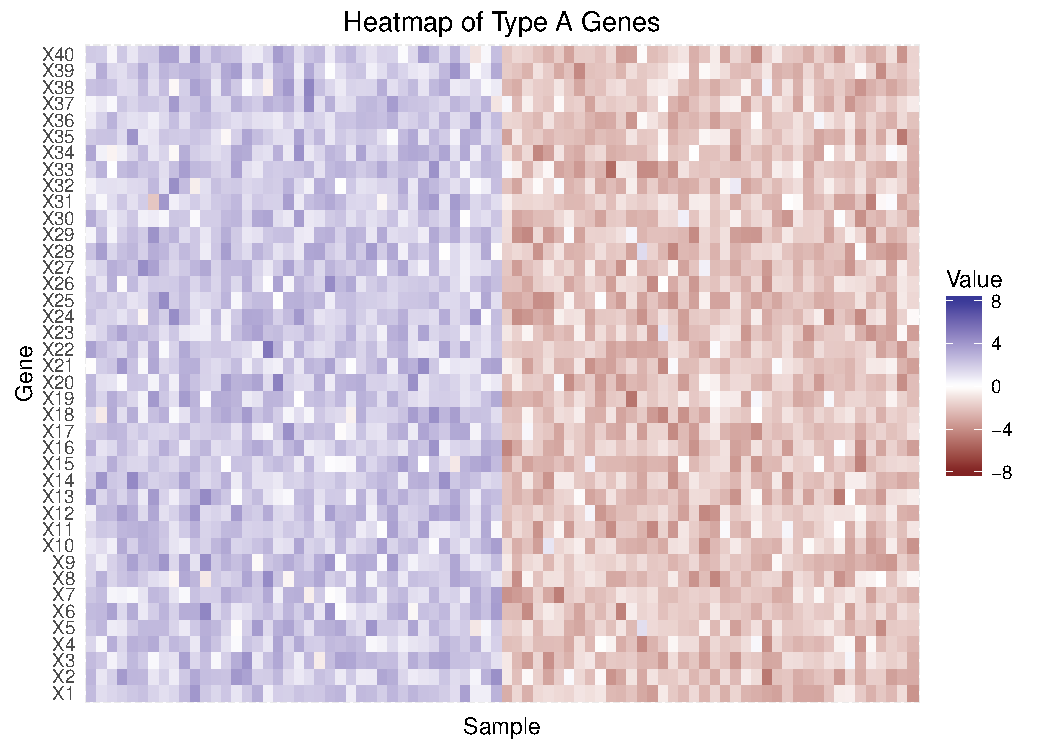
\includegraphics[width = \textwidth]{figures/Type_A_Gene.pdf}
    \caption{Type A: genes associated with class label but not with batch label.}
    \end{subfigure}
    ~
    \centering
    \begin{subfigure}[t]{0.4\textwidth}
    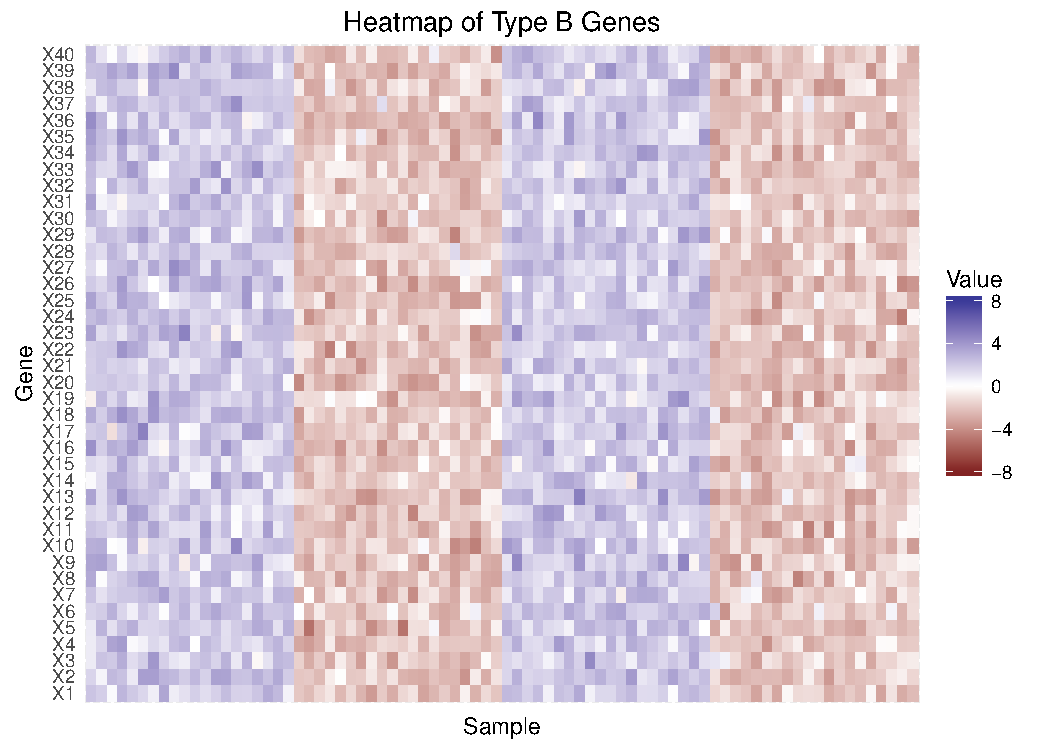
\includegraphics[width = \textwidth]{figures/Type_B_Gene.pdf}
    \caption{Type B: genes associated with batch label but not with class label.}
    \end{subfigure}
    \\
    \centering
    \begin{subfigure}[t]{0.4\textwidth}
    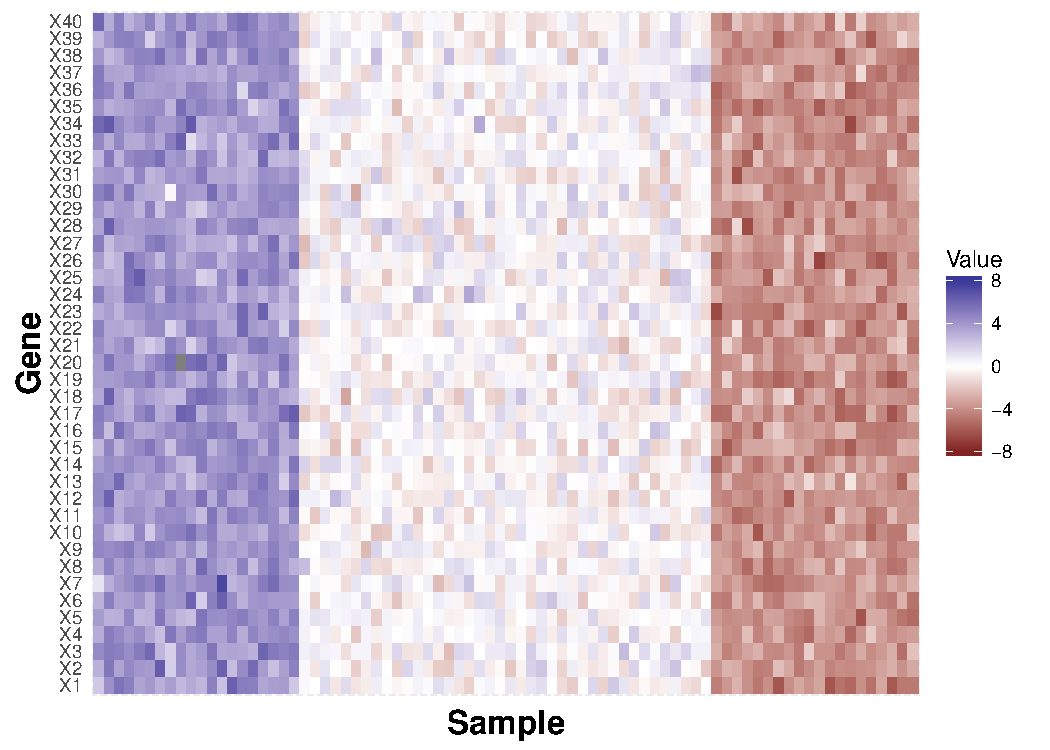
\includegraphics[width = \textwidth]{figures/Type_C_Gene.pdf}
    \caption{Type C: genes associated with both class label and batch label.}
    \end{subfigure}
    ~
    \centering
    \begin{subfigure}[t]{0.4\textwidth}
    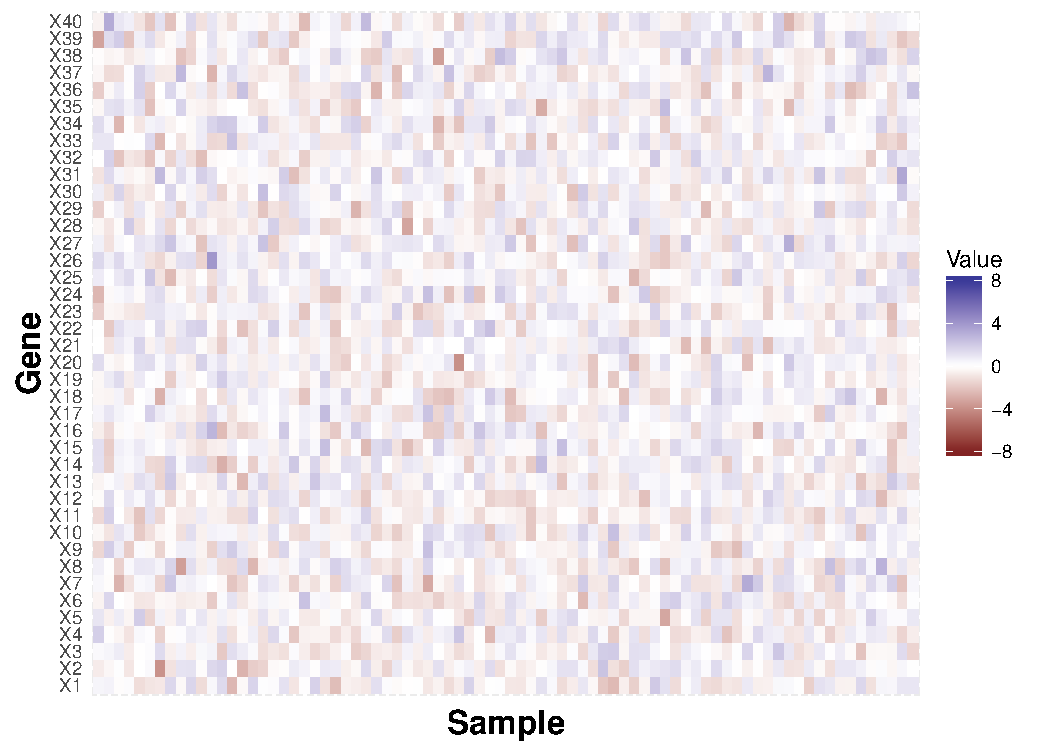
\includegraphics[width = \textwidth]{figures/Type_D_Gene.pdf}
    \caption{Type D: genes containing no signal.}
    \end{subfigure}
    \caption{Heatmap of four types of genes}
    \label{fig:heatmap}
\end{figure}



\newpage
\section{Simulation Result}

\subsection{Case 1: The simulation data set contains only Type C Genes and Type D Genes.}

In the Case 1, Figure~\ref{fig:sva1} shows that IRW-SVA fails to adjust batch effects, while modified SVA adjusts batch effects and recovers the pattern of measured factor pretty well. Figure~\ref{fig:visual1}\subref{fig:pprob1} shows that IRW-SVA can not correctly identify the genes associated with batch label, while modified SVA are able to correctly identify the genes associated with batch label and class label. Moreover, Figure~\ref{fig:visual1}\subref{fig:vector1} shows samples from two batches are more separable under the direction of surrogate variable gained from modified SVA. 

The simulation results in the Case 1 indicate that modified SVA has better performance than IRW-SVA when Type B genes does not exist in the data.

\begin{figure}[h!]
    \centering
    \begin{subfigure}[b]{0.3\textwidth}
        \centering
        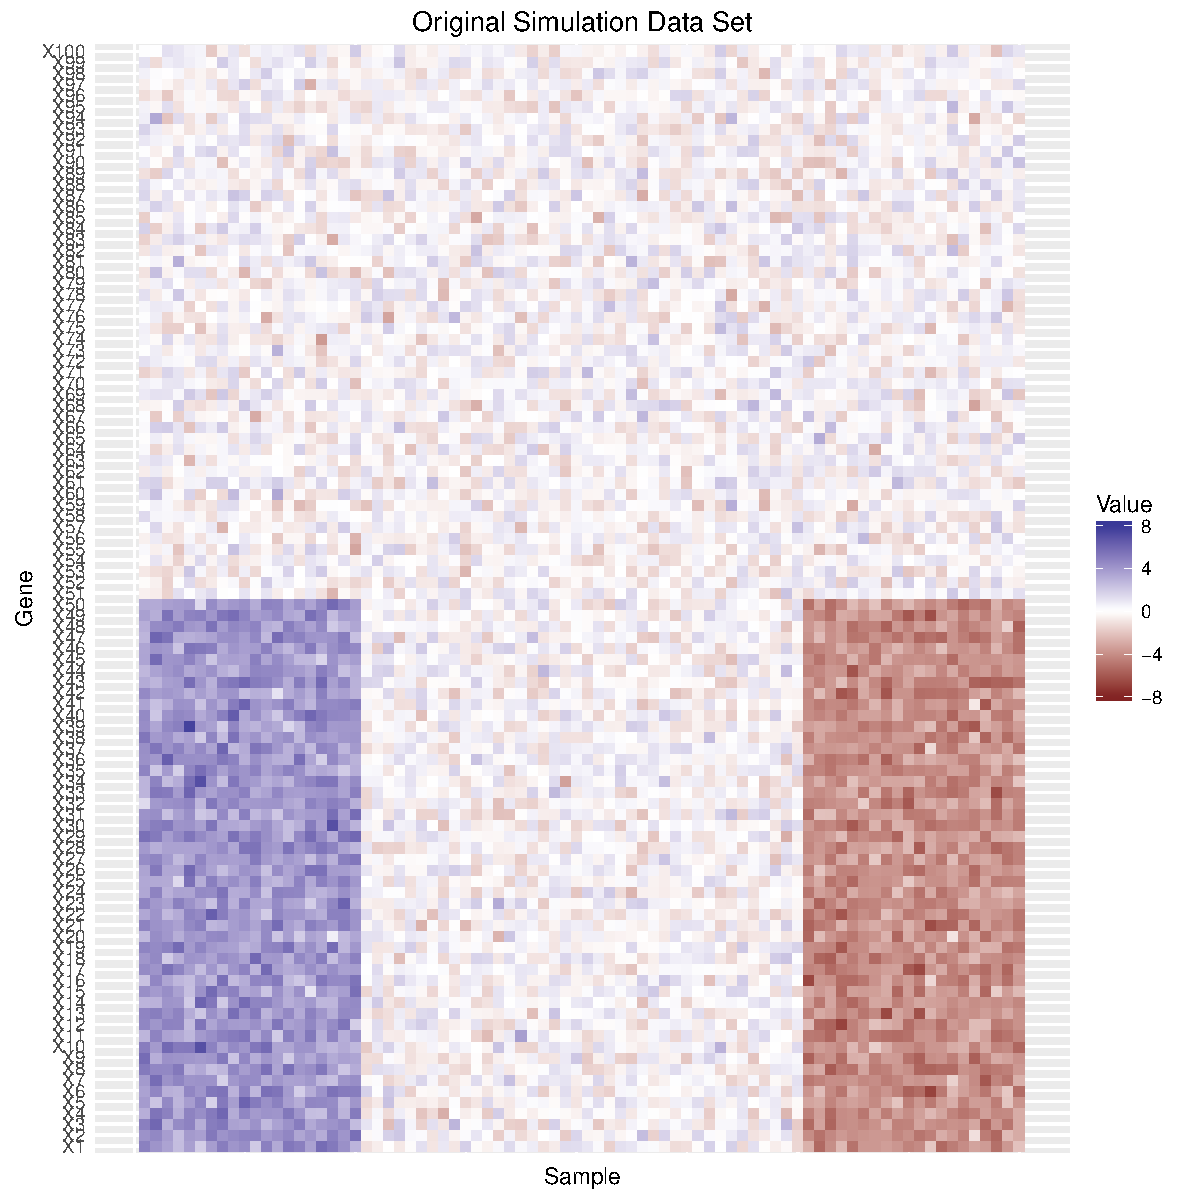
\includegraphics[width = \textwidth]{figures/simulate4.pdf}
        \caption{Original simulation data set in the Case 1}
    \end{subfigure}% 
~
    \begin{subfigure}[b]{0.3\textwidth}
        \centering
        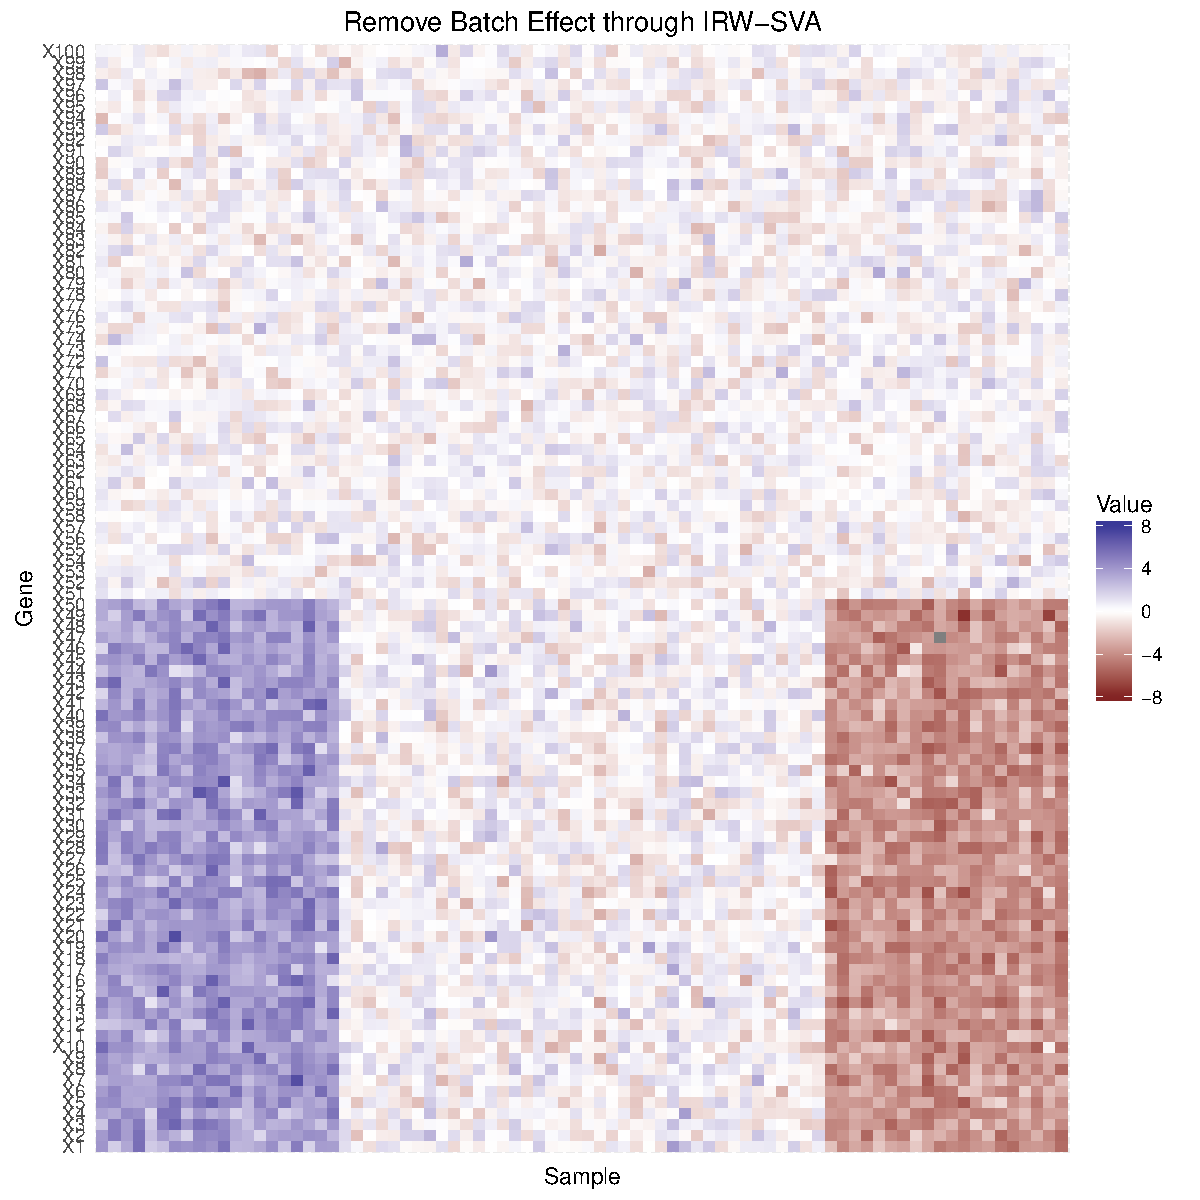
\includegraphics[width = \textwidth]{figures/sva4.pdf}
        \caption{Remove batch effect through IRW-SVA}
    \end{subfigure}  %
~
    \begin{subfigure}[b]{0.3\textwidth}
        \centering
        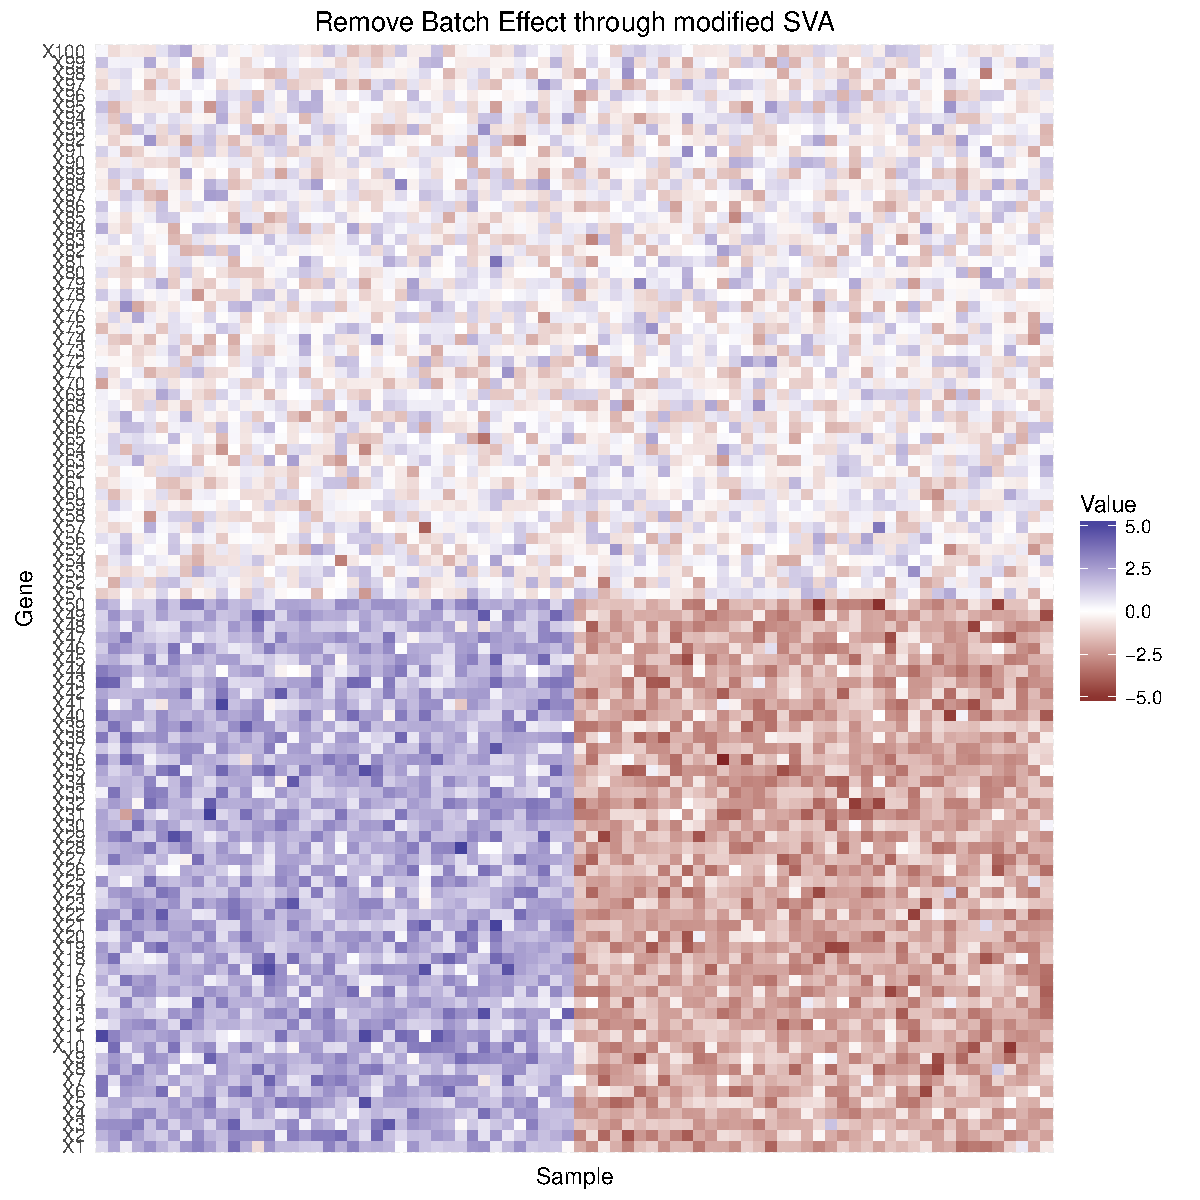
\includegraphics[width = \textwidth]{figures/new_sva4.pdf}
        \caption{Remove batch effect through modified SVA}
    \end{subfigure}    
    \caption{Study batch effect through two approaches to SVA in the case 1}
    \label{fig:sva1}
\end{figure}




\begin{figure}[h!]
    \centering
    \begin{subfigure}[t]{0.4\textwidth}
    \centering
    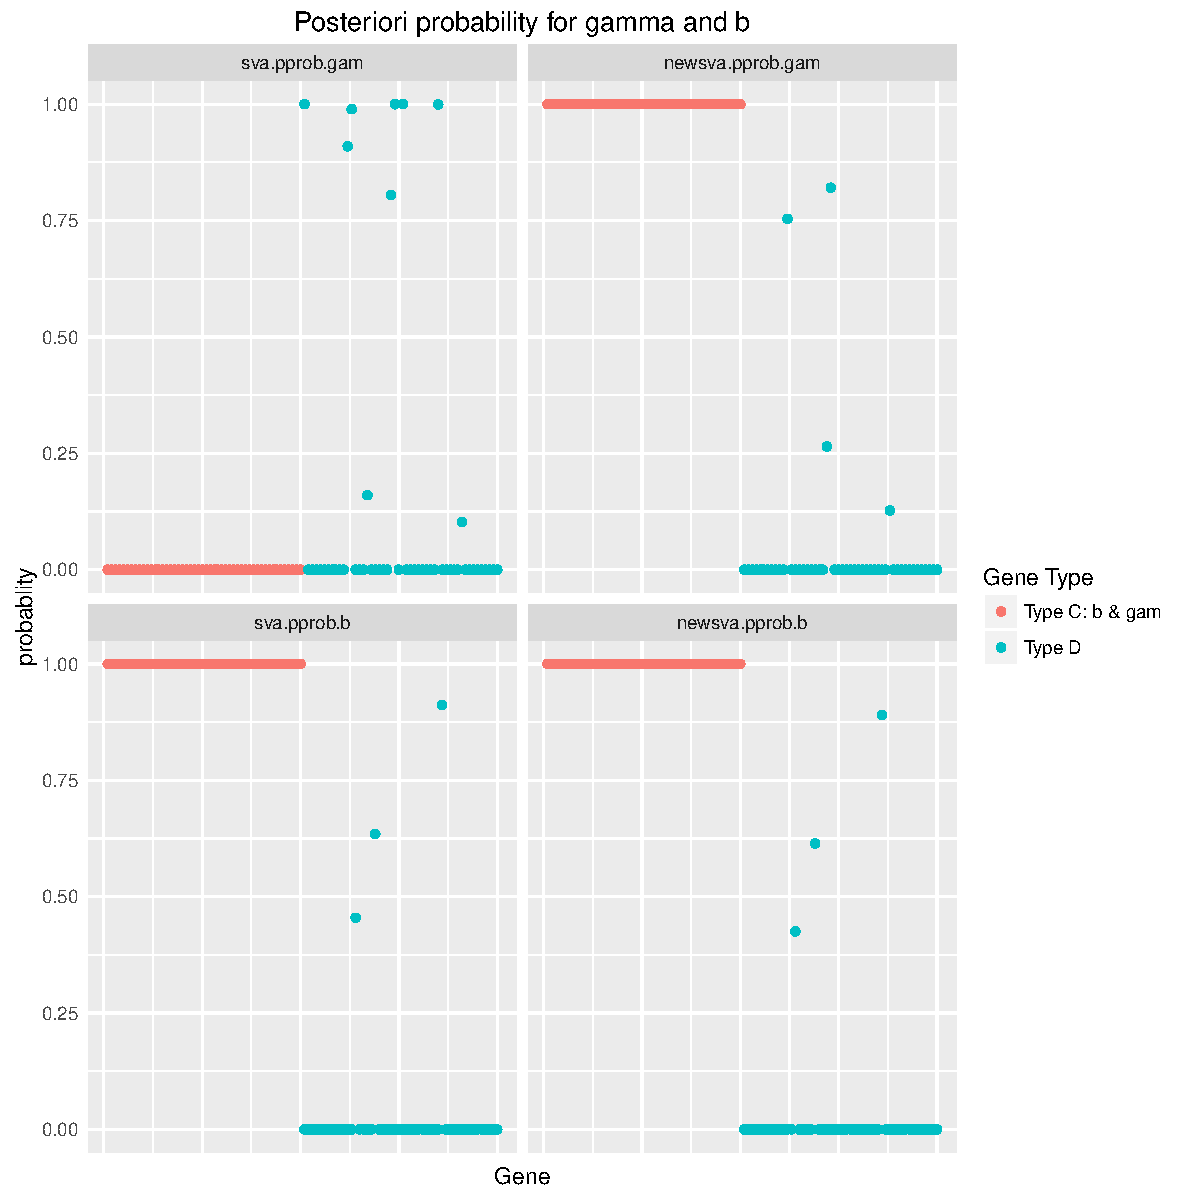
\includegraphics[width = \textwidth]{figures/pprop4.pdf}
    \caption{pprob.b: posterior probability of genes affected by measured factor.\\
    pprob.gam: posterior probability of genes affected by unmeasured factor.}
    \label{fig:pprob1}
    \end{subfigure}
~    
    \begin{subfigure}[t]{0.4\textwidth}
    \centering
    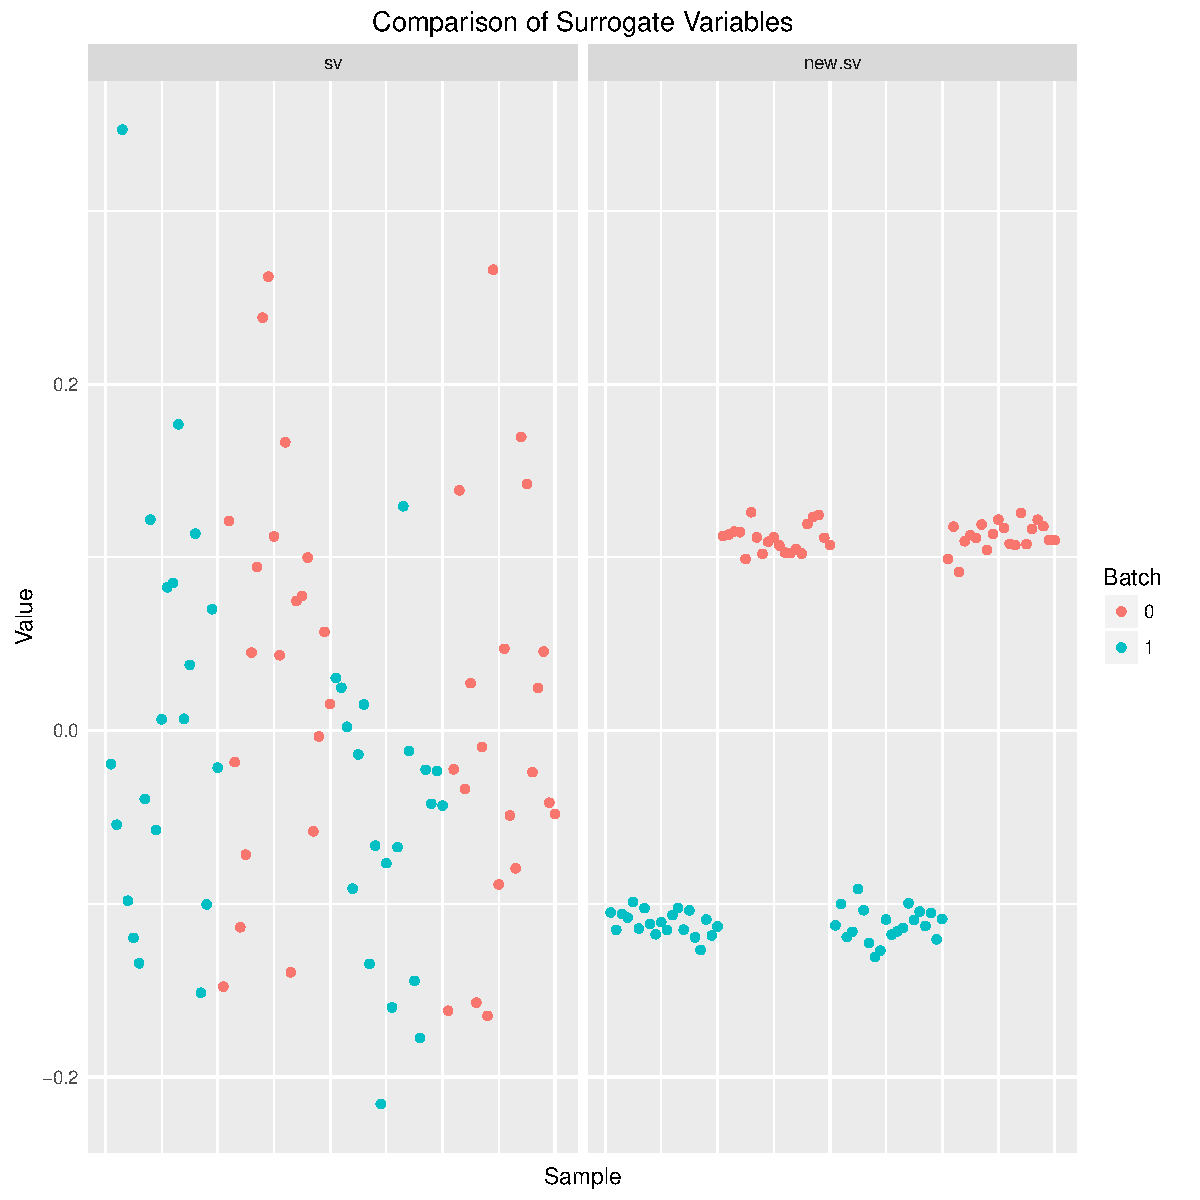
\includegraphics[width = \textwidth]{figures/vector4.pdf}
    \caption{Comparison of surrogate variables}
    \label{fig:vector1}
    \end{subfigure}
    \caption{Visualize the analysis through sample space and gene space in the Case 1. In each subfigure, the panels on the left show the results from IRW-SVA and the panels on the right show the results form modified SVA.}
    \label{fig:visual1}
\end{figure}


\newpage

\subsection{Case 2: The simulation data set contains all four types of genes.}

Figure~\ref{fig:sva2} shows that both IRW-SVA and modified SVA can adjust the batch effects in the Case 2.  Figure~\ref{fig:visual2}\subref{fig:pprob2} shows that both IRW-SVA and modified SVA are able to identify the genes associated with batch label and class label. Figure~\ref{fig:visual2}\subref{fig:vector2} shows that they produce similar surrogate variable which separate samples from two batches pretty well.

The simulation results in the Case 2 indicate that IRW-SVA and modified SVA have similar performance when the data set contains Type B genes.

\begin{figure}[h!]
    \centering
    \begin{subfigure}[b]{0.3\textwidth}
        \centering
        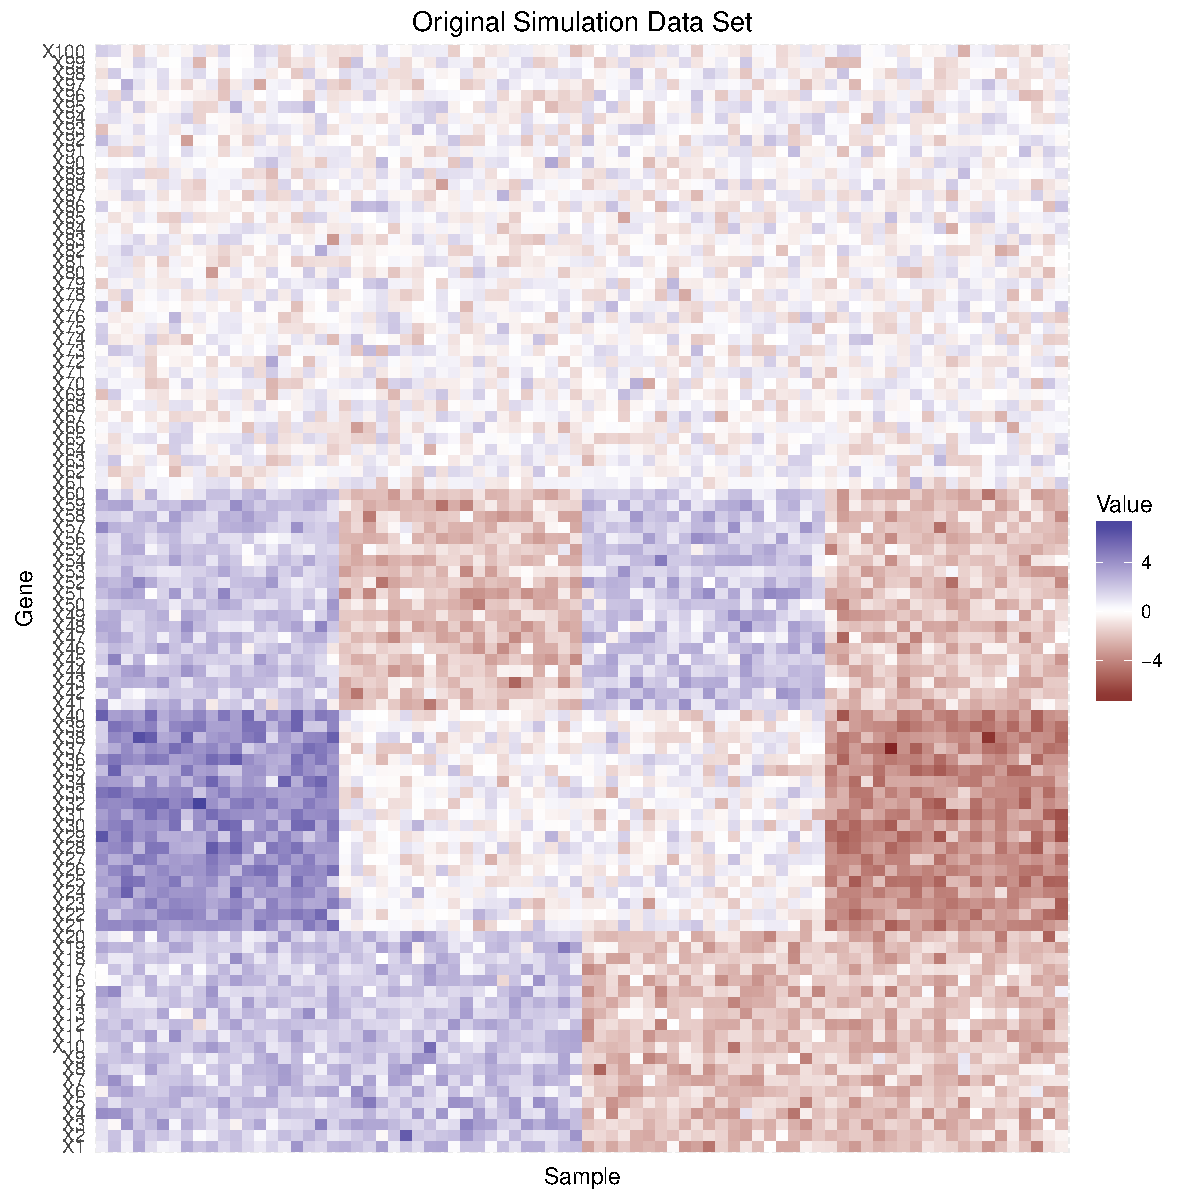
\includegraphics[width = \textwidth]{figures/simulate0.pdf}
        \caption{Original simulation data set in the Case 2}
    \end{subfigure}% 
~
    \begin{subfigure}[b]{0.3\textwidth}
        \centering
        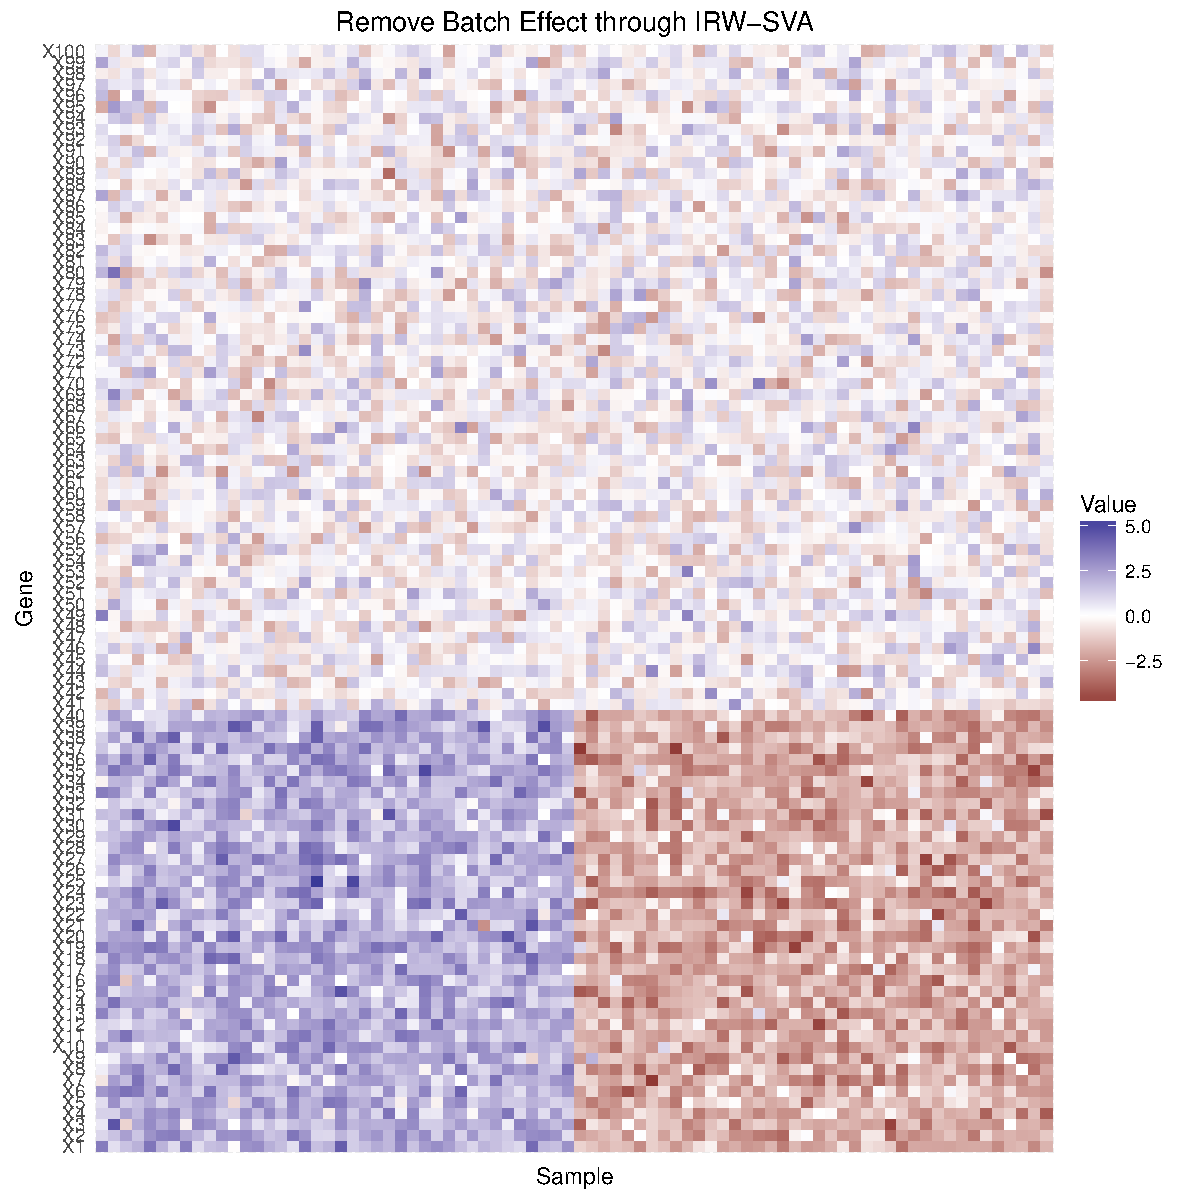
\includegraphics[width = \textwidth]{figures/sva0.pdf}
        \caption{Remove batch effect through IRW-SVA}
    \end{subfigure}  %
~
    \begin{subfigure}[b]{0.3\textwidth}
        \centering
        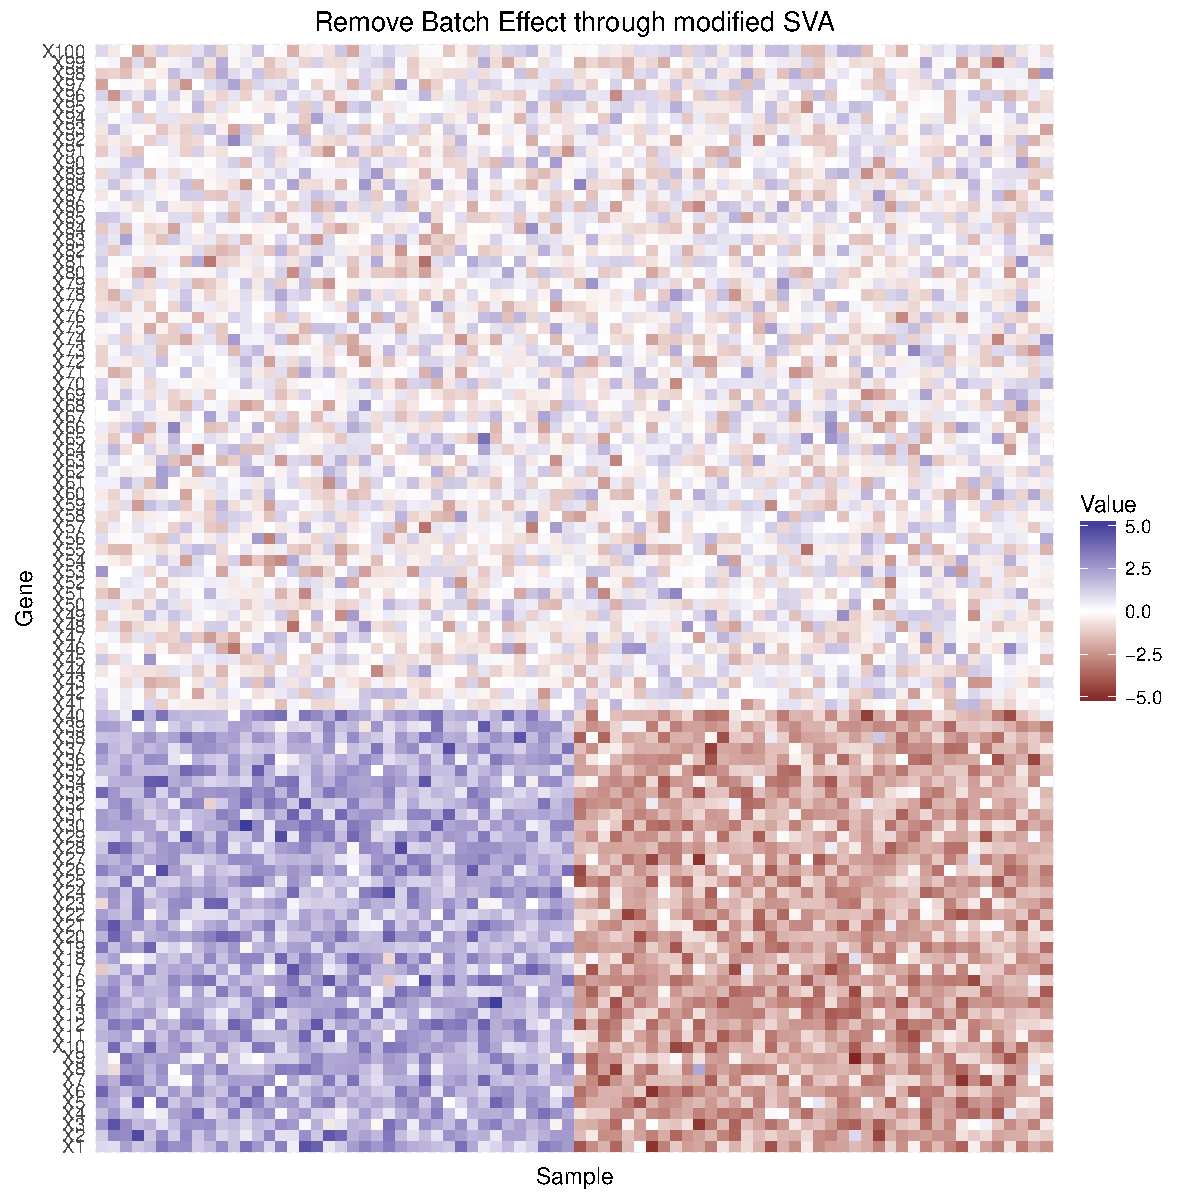
\includegraphics[width = \textwidth]{figures/new_sva0.pdf}
        \caption{Remove batch effect through modified SVA}
    \end{subfigure}    
    \caption{Study batch effect through two approaches to SVA in the Case 2}
    \label{fig:sva2}
\end{figure}


\begin{figure}[h!]
    \centering
    \begin{subfigure}[t]{0.4\textwidth}
    \centering
    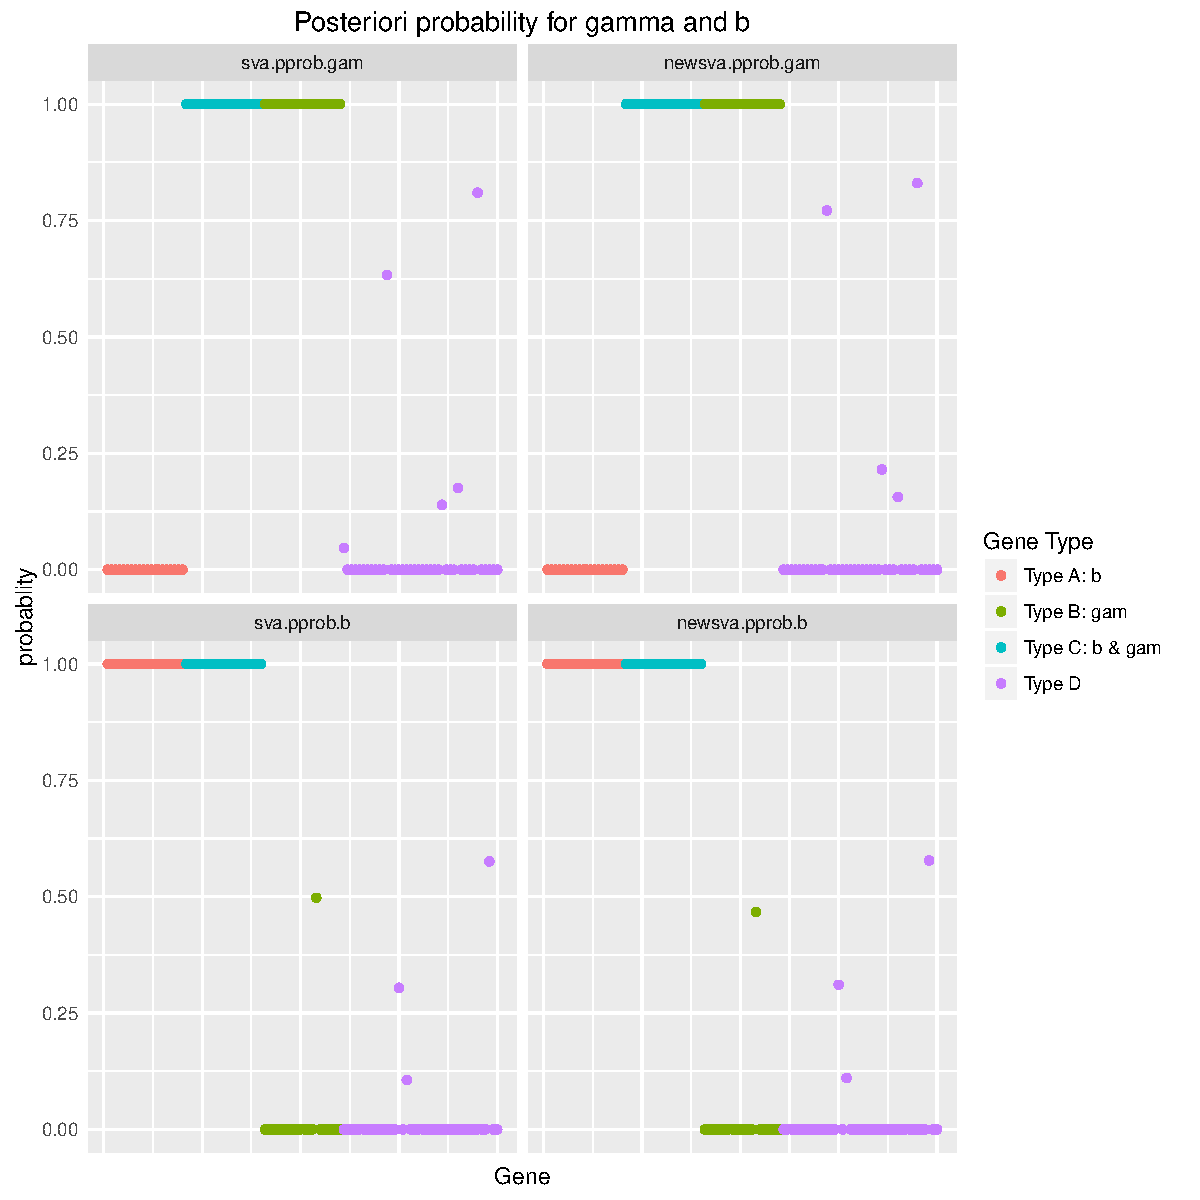
\includegraphics[width = \textwidth]{figures/pprop0.pdf}
    \caption{pprob.b: posterior probability of genes affected by measured factor.\\
    pprob.gam: posterior probability of genes affected by unmeasured factor.}
    \label{fig:pprob2}
    \end{subfigure}
~    
    \begin{subfigure}[t]{0.4\textwidth}
    \centering
    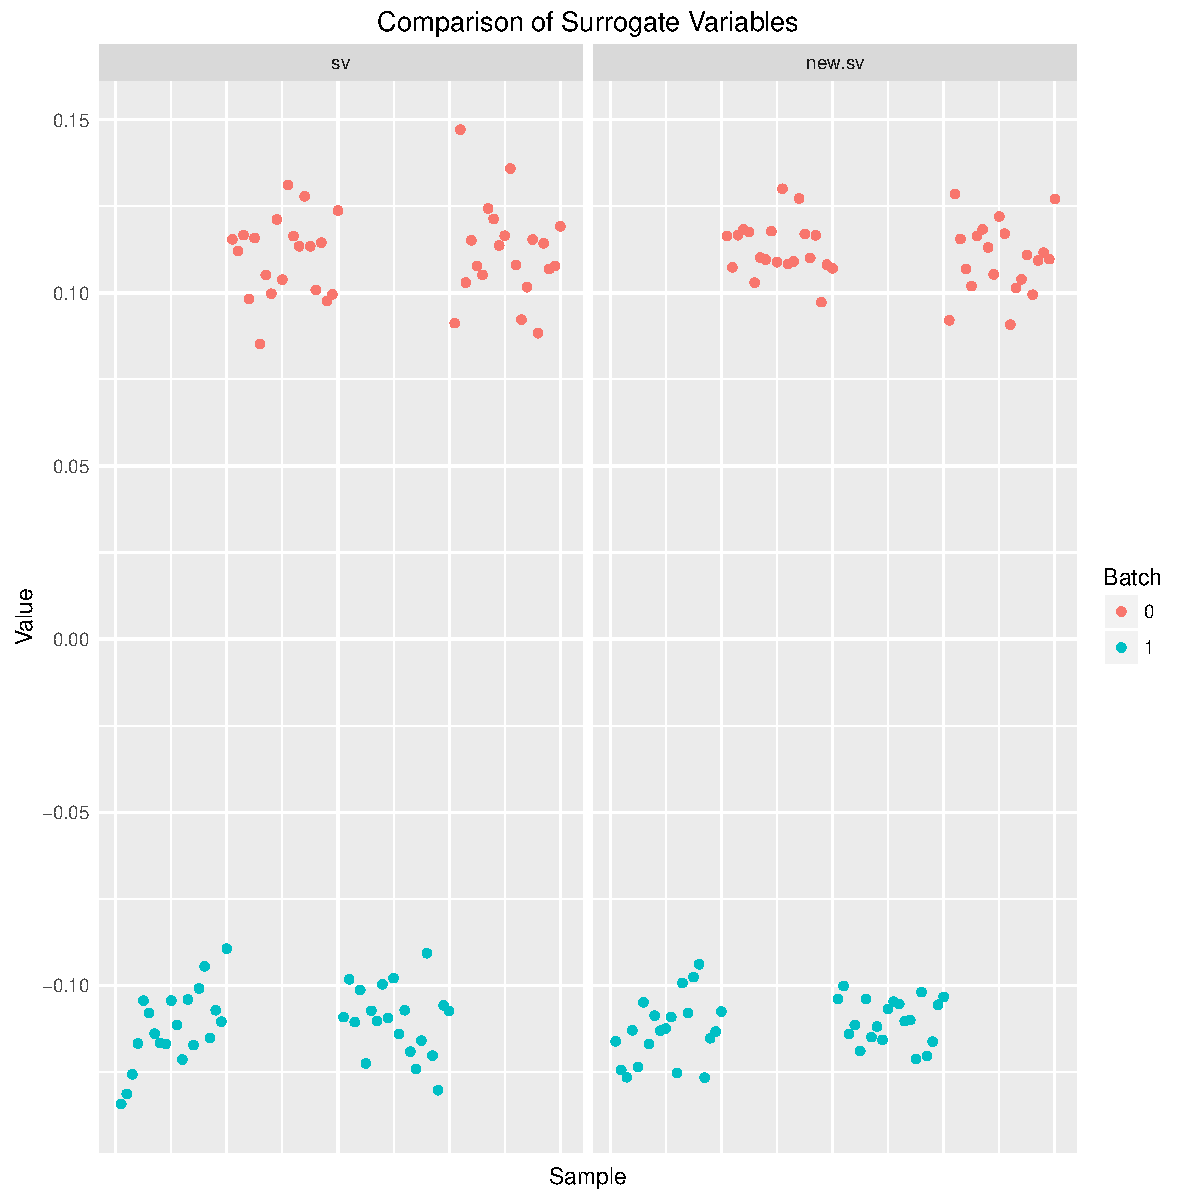
\includegraphics[width = \textwidth]{figures/vector0.pdf}
    \caption{Comparison of surrogate variables}
    \label{fig:vector2}
    \end{subfigure}
    \caption{Visualize the analysis from sample space and gene space in the Case 2. In each subfigure, the panels on the left show the results from IRW-SVA and the panels on the right show the results form modified SVA.}
     \label{fig:visual2}
\end{figure}

\newpage
\clearpage

\bibliographystyle{plain}
\bibliography{svabib}

\end{document}